\section{K-Means Clustering}
\label{sec:K-Means}
The K-Means algorithm detects the clusters / partitions by measuring the euclidean distance between the cluster centroids and the position of the street junctions \cite{k-means++:2007}. The algorithm uses the following approach:

\begin{enumerate}
    \item A number of points are inserted randomly into the graph and used as centroids.
    \item All graph points are assigned to their nearest centroids.
    \item The centroids are moved to the center of their assigned graph points.
    \item Until the maximum number of iterations is reached this process is repeated starting by loop item 2.
\end{enumerate}

\subsection{Local minima problem}
Because the K-Means algorithm can find local minima, this process needs to be executed more than once. The result with the best found solution will be selected.

\subsection{K-Means++}
The K-Means algorithm was later extended to set reasonable start centroids. This extensions allows to run a K-Means run with $O(log\ k)$ \cite{k-means++:2007}.

\pagebreak
\FloatBarrier
\section{Hierarchical Clustering} 
\label{sec:hierarchicalClustering}
\subsection{Introduction}
Hierarchical clustering is also known as connectivity based clustering. This area of algorithms clusters nodes together, which are near to each other. The advantage over K-Means is that graph distances can be used instead of the euclidean distance.

The result of a hierarchical clustering algorithm is a tree (or hierarchy), hence the name. This result can be used to create 1 to n clusters, where n is the number of input nodes.

\subsection{Strategy}
There are generally two main strategies for hierarchical clustering:

\begin{itemize}
    \item \textbf{Agglomerative}: Bottom up strategy. In the beginning each node is an own cluster. Clusters are combined until only a single cluster remains.
    \item \textbf{Divisive}: Top down strategy. All nodes are contained in one cluster at the start. This cluster is then divided into sub clusters.
\end{itemize}

The time complexity of the divisive strategy with $O(2^n)$ is not performing well enough for the size of the street networks on which the algorithms have to run. The agglomerative strategy runs in $O(n^2 log(n))$ and in some special cases in $O(n^2)$ time complexity. The hierarchical clustering algorithms implemented for this thesis run in $O(n^2)$ time complexity. They are based on the paper "Optimal implementations of UPGMA and other common clustering algorithms" \cite{clustering:2007}.

\subsection{Reduction Formula}
The reduction formula is used to determine the distance between two clusters.
The following reduction formulae were implemented for this thesis:

\begin{itemize}
    \item \textbf{Single Linkage}
    \begin{multline}
    D_{Single-Linkage}(C_1, (C_2 \cup C_3)) \leftarrow \\
    min \{ D_{Single-Linkage}(C_1, C_2), D_{Single-Linkage}(C_1, C_3) \}
    \end{multline}
    \item \textbf{\acrshort{UPGMA}} (\acrlong{UPGMA})
    \begin{equation}
    \begin{split}
    D_{UPGMA}(C_1, (C_2 \cup C_3)) \leftarrow &\frac{|C_2|}{|C_2|+|C_3|}D_{UPGMA}(C_1, C_2)\ + \\ &\frac{|C_3|}{|C_2|+|C_3|}D_{UPGMA}(C_1, C_3)
    \end{split}
    \end{equation}
    \item \textbf{\acrshort{WPGMA}} (\acrlong{WPGMA})
    \begin{equation}
    D_{WPGMA}(C_1, (C_2 \cup C_3)) \leftarrow \frac{1}{2} (D_{WPGMA}(C_1, C_2) + D_{WPGMA}(C_1, C_3))
    \end{equation}
\end{itemize}

$C_1$, $C_2$ and $C_3$ are clusters, each being a set of nodes. The distance function $d(i, j)$ determines the distance between nodes $i$ and $j$.

For every of these reduction formulae the following holds:

\begin{equation}
\begin{split}
&\textrm{let }C_1, C_2\textrm{ be clusters}, i \in C_1, j \in C_2 \\
&\textrm{if }|C_1| = |C_2| = 1 \\
&\textrm{then }D(C_1, C_2) = d(i, j)
\end{split}
\end{equation}

For both the single linkage and the \acrshort{UPGMA} reduction formula exists a dissimilarity function (\ref{eq:df_single_linkage} and \ref{eq:df_upgma}). These are alternative formulations of the reduction formulae which determine the cluster distance by traversing all nodes of both clusters. The created cluster hierarchy is not used in these functions. For the \acrshort{WPGMA} reduction formula no dissimilarity function exists, as shown in \cite{clustering:2007}.

\begin{align}
\label{eq:df_single_linkage}
D_{Single-Linkage}(C_1, C_2) &= \min_{i\in{C1}, j\in{C2}}\{d(i, j)\} \\
\label{eq:df_upgma}
D_{UPGMA}(C_1, C_2) &= \dfrac{1}{|C_1||C_2|} \sum_{i\in{C1}, j\in{C2}}{d(i, j)}
\end{align}

\subsection{Hierarchy}
The output of the hierarchical clustering algorithm is as the name suggests a hierarchy. Figure \ref{fig:hierarchy} shows such an output. For simplicity only five input nodes were used. If this hierarchy was created using an agglomerative strategy the result could have been built as follows:

\begin{enumerate}
    \item Combine the two leftmost nodes
    \item Combine the two rightmost nodes
    \item Combine the cluster formed in step 1 with the middle node
    \item Combine the cluster formed in step 3 with the one combined in step 2
\end{enumerate}

To create a clustering from this output the procedure from above is reversed. In the order, in which the combinations were made, the clusters are split. The hierarchy can be looked at as a single cluster. With each split one hierarchy is divided into two new hierarchies.

Using this method it is possible to create 1 to $n$ clusters from any hierarchy, where $n$ is the number of nodes. Figure \ref{fig:hierarchy_with_clusters} shows an example of this process. From the same hierarchy with five nodes which was used before two clusters were created. A later section (\ref{sec:outout_modification}) shows, that the order in which the hierarchies are split, can be modified.

\begin{figure}[!hb]
    \centering
    \begin{subfigure}[b]{\textwidth}
        \begin{mdframed}[style=border]
            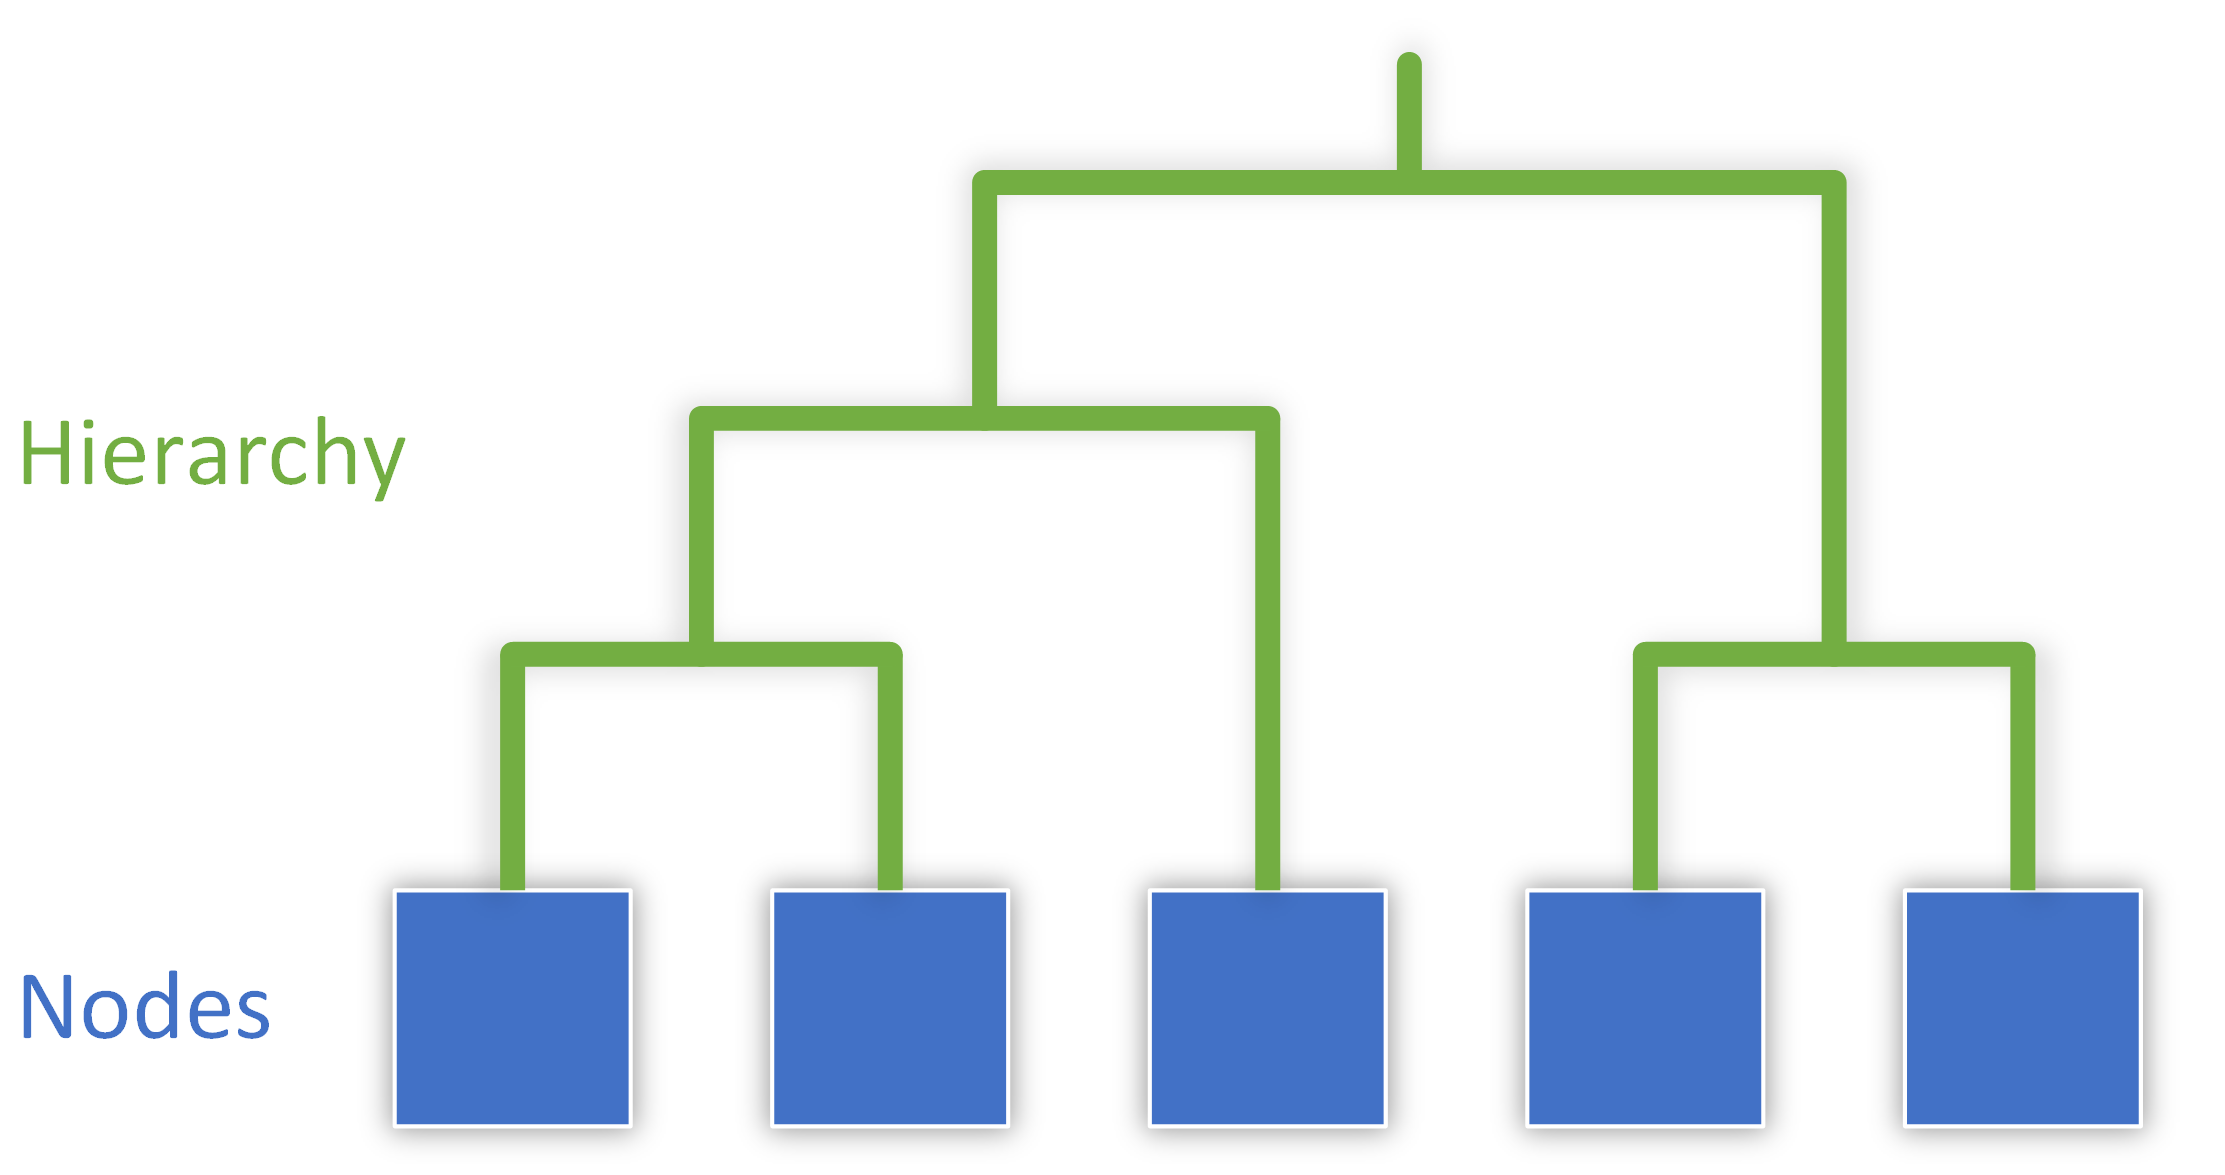
\includegraphics[width=\linewidth]{hierarchy.png}
        \end{mdframed}
        \caption{Hierarchy, which is the output of a hierarchical clustering algorithm}
        \label{fig:hierarchy}
    \end{subfigure}
    \par\medskip
    \begin{subfigure}[b]{\textwidth}
        \begin{mdframed}[style=border]
            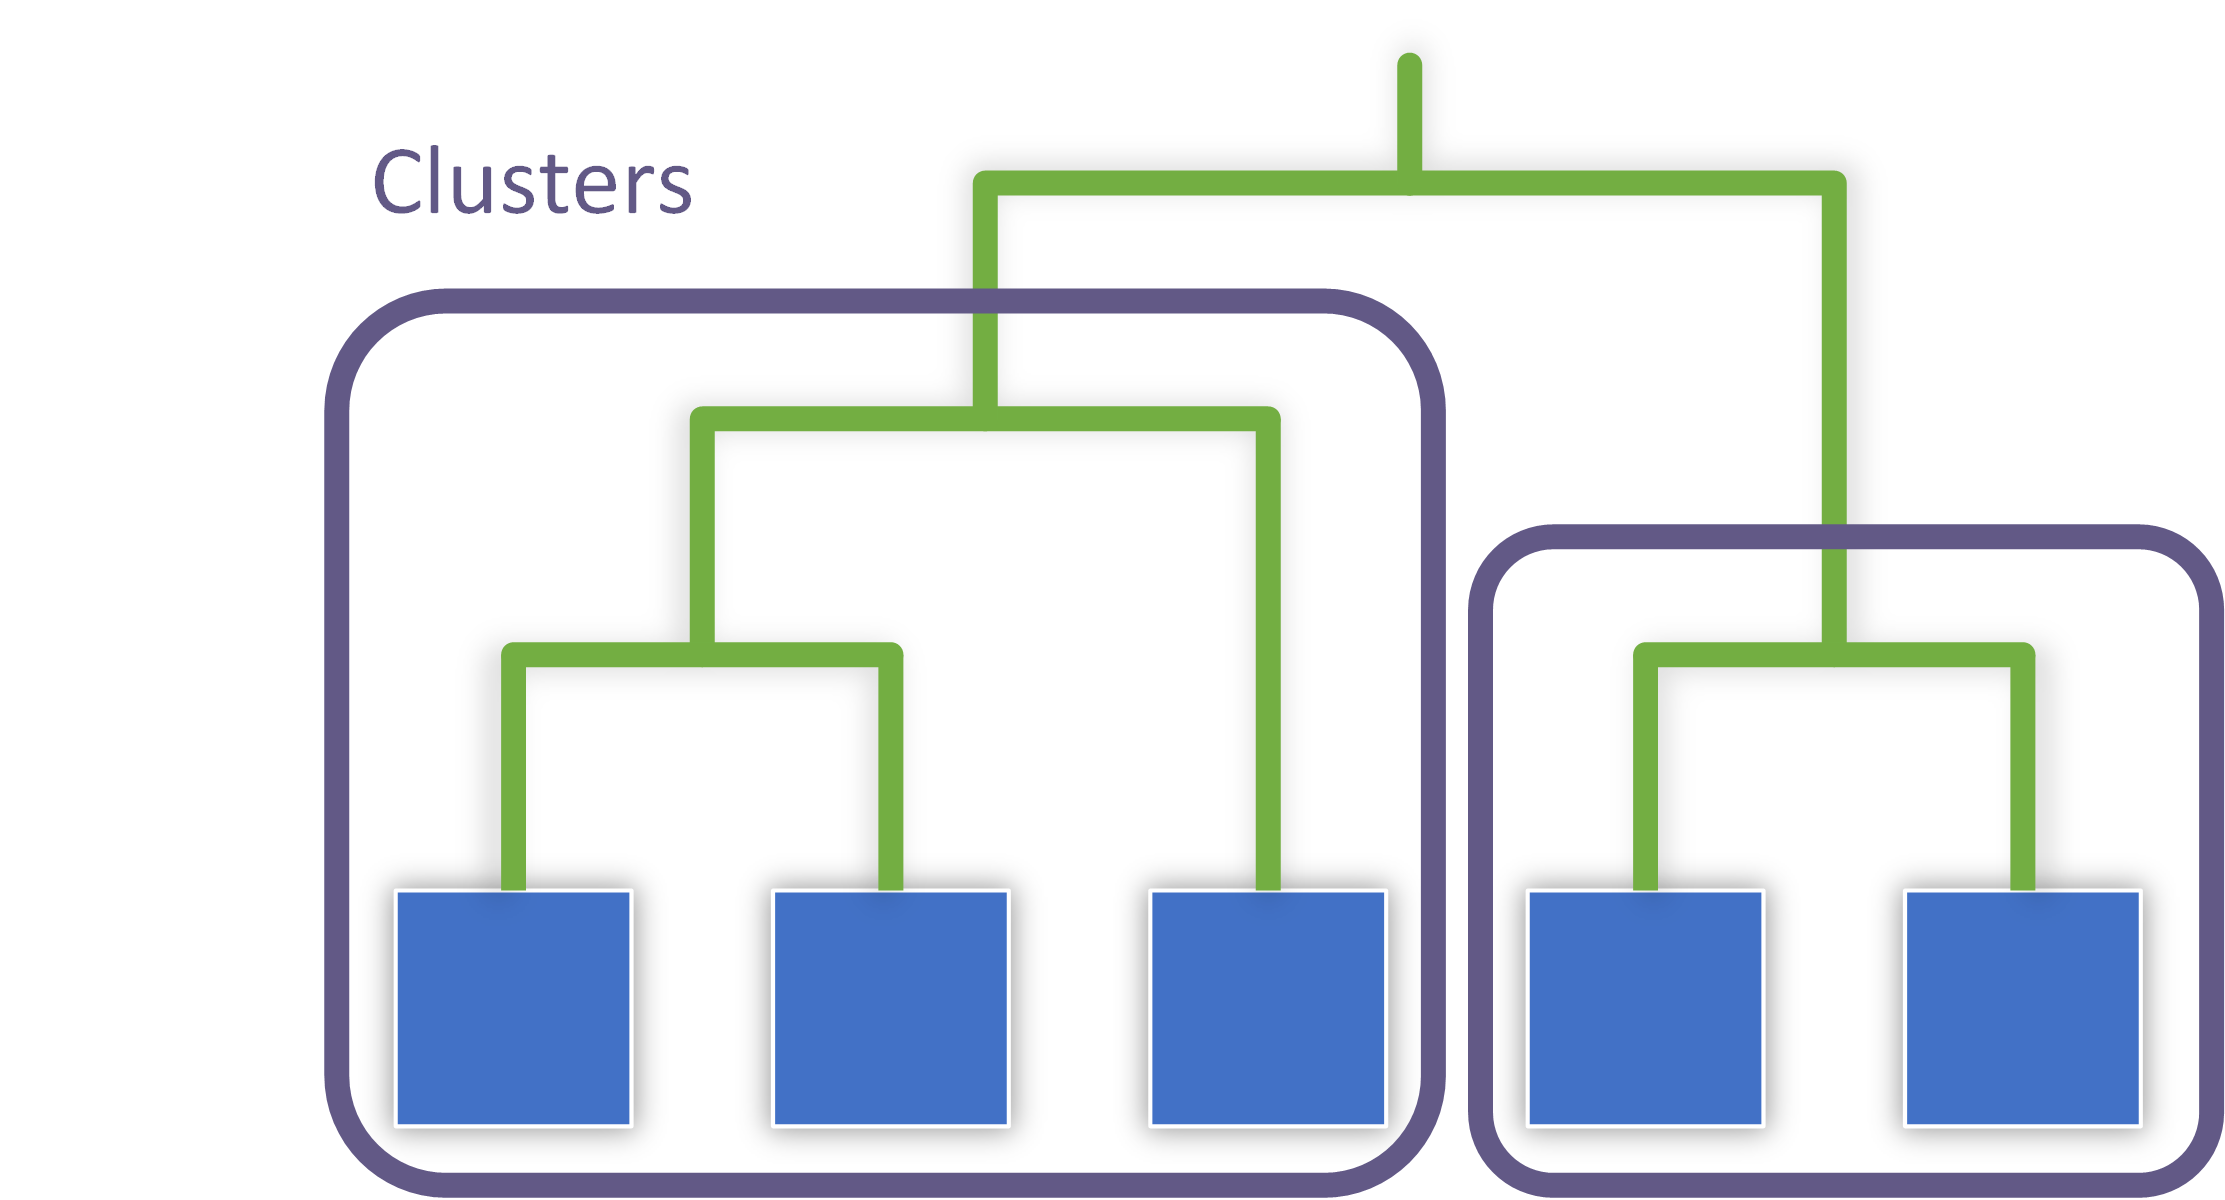
\includegraphics[width=\linewidth]{hierarchy_with_clusters.png}
        \end{mdframed}
        \caption{Example of two clusters created from the hierarchy}
        \label{fig:hierarchy_with_clusters}
    \end{subfigure}
    \caption{Visualisation of the output of hierarchical clustering algorithms}
\end{figure}


\section{Cluster Analysis}
\label{sec:clusterRating}
To evaluate the generated clusters different measurement methods are necessary. Jun. Prof. Dr.  Reinhard König from the ETH Zurich proposed the following parameters.
\newline
\begin{itemize}
    \item Geometry based measurements:
    \begin{itemize}
        \item Area based on the convex hull of the cluster area
        \item Total length of the streets
        \item Ratio between the area and total length
        \item Distribution variance of the street length
        \item Distribution variance of the street angles
        \item Ratio between street block size and surrounding circle area (minima, maxima, mean)
    \end{itemize}
    \item Centrality-based measurements normalized by the street count (minima, maxima, mean):
    \begin{itemize}
        \item In-Centrality (Integration)
        \item In-Betweenness-Centrality (Choice)
    \end{itemize}
\end{itemize}
The centrality based ratings and the block area calculation were pre implemented in CPlan \ref{CPlan}. Additional a GUI to compared and stored the results as JSON-File for each generated cluster has been added.

Some initial measurements and comparisons are made in the cluster analysis chapter \ref{sec:measurements-cluster-analysis}.

\subsection{Block Area Ratio}
In the paper \textit{A typology of street patterns}\citep{blockArea:2014} the method is described how cities/areas can be classified and compared by analysing the block areas instead of the streets. First the block area is calculated and then the result is divided by the circumscribed circle area.

\subsection{Centrality}
The parameter \textit{Integration} describes the closeness centrality. This means the normed sum of the distances from all other vertex based on te shortest path algorithm is calculated. The vertex with the lowest value must be the most central.

With \textit{Choice} the betweenness centrality is described. The approach is to calculate the shortest path between every vertex. Every time a given vertex is visited the betweenness-centrality value of the vertex is raised by one. As a result the highest measured value indicates for a vertex to be in or near the centre of a graph.

\subsection{Variance}
The parameter variance describes the sigma of the normal curve of the distribution function.
First of all the measured data is round to fit into a distribution function \ref{eq:distribution_function}. Then the expected value \ref{eq:expected_value} and the variance \ref{eq:variance} is calculated. Finally the standard deviation (square root of V(x)) is computed \ref{eq:standard_deviation}.
\begin{align}
\label{eq:distribution_function} 
F(x) &= P(X \leq x) =  \sum_{t\in{X}, t\leq{x}}{f(t)} \\
\label{eq:expected_value} 
E(x) &= \int\limits_{-\infty}^\infty x * f(x)dx \\
\label{eq:variance} 
V(x) &= \int\limits_{-\infty}^\infty (x - E(X))^2 * f(x)dx \\
\label{eq:standard_deviation} 
\sigma(x) &= \sqrt{V(x)}
\end{align}

\section{All Pairs Shortest Path} \label{sec:shortest_path}
%TODO rewrite
As already stated, the implementations of hierarchical clustering algorithms developed during this thesis use graph distances. The calculation of the shortest path between two nodes every time it is needed would not be viable, because these distances have to be accessed multiple times. So it is necessary to calculate and store them in advance using an \gls{APSP} algorithm.
